%\documentclass[handout]{ximera}
\documentclass[nooutcomes]{ximera}

\usepackage{gensymb}
\usepackage{tabularx}
\usepackage{mdframed}
\usepackage{pdfpages}
%\usepackage{chngcntr}

\let\problem\relax
\let\endproblem\relax

\newcommand{\property}[2]{#1#2}




\newtheoremstyle{SlantTheorem}{\topsep}{\fill}%%% space between body and thm
 {\slshape}                      %%% Thm body font
 {}                              %%% Indent amount (empty = no indent)
 {\bfseries\sffamily}            %%% Thm head font
 {}                              %%% Punctuation after thm head
 {3ex}                           %%% Space after thm head
 {\thmname{#1}\thmnumber{ #2}\thmnote{ \bfseries(#3)}} %%% Thm head spec
\theoremstyle{SlantTheorem}
\newtheorem{problem}{Problem}[]

%\counterwithin*{problem}{section}



%%%%%%%%%%%%%%%%%%%%%%%%%%%%Jenny's code%%%%%%%%%%%%%%%%%%%%

%%% Solution environment
%\newenvironment{solution}{
%\ifhandout\setbox0\vbox\bgroup\else
%\begin{trivlist}\item[\hskip \labelsep\small\itshape\bfseries Solution\hspace{2ex}]
%\par\noindent\upshape\small
%\fi}
%{\ifhandout\egroup\else
%\end{trivlist}
%\fi}
%
%
%%% instructorIntro environment
%\ifhandout
%\newenvironment{instructorIntro}[1][false]%
%{%
%\def\givenatend{\boolean{#1}}\ifthenelse{\boolean{#1}}{\begin{trivlist}\item}{\setbox0\vbox\bgroup}{}
%}
%{%
%\ifthenelse{\givenatend}{\end{trivlist}}{\egroup}{}
%}
%\else
%\newenvironment{instructorIntro}[1][false]%
%{%
%  \ifthenelse{\boolean{#1}}{\begin{trivlist}\item[\hskip \labelsep\bfseries Instructor Notes:\hspace{2ex}]}
%{\begin{trivlist}\item[\hskip \labelsep\bfseries Instructor Notes:\hspace{2ex}]}
%{}
%}
%% %% line at the bottom} 
%{\end{trivlist}\par\addvspace{.5ex}\nobreak\noindent\hung} 
%\fi
%
%


\let\instructorNotes\relax
\let\endinstructorNotes\relax
%%% instructorNotes environment
\ifhandout
\newenvironment{instructorNotes}[1][false]%
{%
\def\givenatend{\boolean{#1}}\ifthenelse{\boolean{#1}}{\begin{trivlist}\item}{\setbox0\vbox\bgroup}{}
}
{%
\ifthenelse{\givenatend}{\end{trivlist}}{\egroup}{}
}
\else
\newenvironment{instructorNotes}[1][false]%
{%
  \ifthenelse{\boolean{#1}}{\begin{trivlist}\item[\hskip \labelsep\bfseries {\Large Instructor Notes: \\} \hspace{\textwidth} ]}
{\begin{trivlist}\item[\hskip \labelsep\bfseries {\Large Instructor Notes: \\} \hspace{\textwidth} ]}
{}
}
{\end{trivlist}}
\fi


%% Suggested Timing
\newcommand{\timing}[1]{{\bf Suggested Timing: \hspace{2ex}} #1}




\hypersetup{
    colorlinks=true,       % false: boxed links; true: colored links
    linkcolor=blue,          % color of internal links (change box color with linkbordercolor)
    citecolor=green,        % color of links to bibliography
    filecolor=magenta,      % color of file links
    urlcolor=cyan           % color of external links
}

\title{Reading Information from a Graph}

\author{Vic Ferdinand, Bart Snapp, and Brad Findell}

\outcome{Learning outcome goes here.}

\begin{document}
\begin{abstract}
  We analyze graphs of functions.
\end{abstract}
\maketitle


\begin{teachingnote}
Supplies:  tracing paper (for shifts and reflections).  
Students have little trouble with a through c.  Then discussion is needed. 
\end{teachingnote}

On the next page is the graph of a function called $h(t)$, which
represents the distance (in miles) and direction (east = positive,
west = negative) Johnny is from home $t$ hours after noon. It does not
have a simple formula, so don't try to find one. Answer the following
questions about $h$, briefly explaining how you obtained your
answer(s):

\begin{problem}
On the given graph of $h$, what are the least and greatest values
of $t$? What are the least and greatest values of $h(t)$? What do
these answers say about Johnny?
\end{problem}

\begin{problem}
Evaluate the following expressions: $h(0)$, $h(3)$, and $h(-3)$. What
do each of these say about Johnny? 
\end{problem}

\begin{problem}
For each of the following, solve for $t$ (i.e., find all the values of
$t$ that make the statement true). Describe what you did with the
graph to determine the solutions.  Where possible, interpret
the statement and its solutions in terms of Johnny.

\begin{enumerate}
\item $h(t) = 0$
\item $h(t) = 3$
\item $h(t) \leq 3$
\item $h(t) = h(4.5)$
\item $h(t) = t$
\item $h(t) = -t$
\item $h(t) = h(-t)$
\item $h(t) = -h(-t)$
\item $h(t+1) = h(t)$
\item $h(t)+1 = h(t)$
\end{enumerate}
\end{problem}

\newpage


\resizebox{\textwidth}{!}{
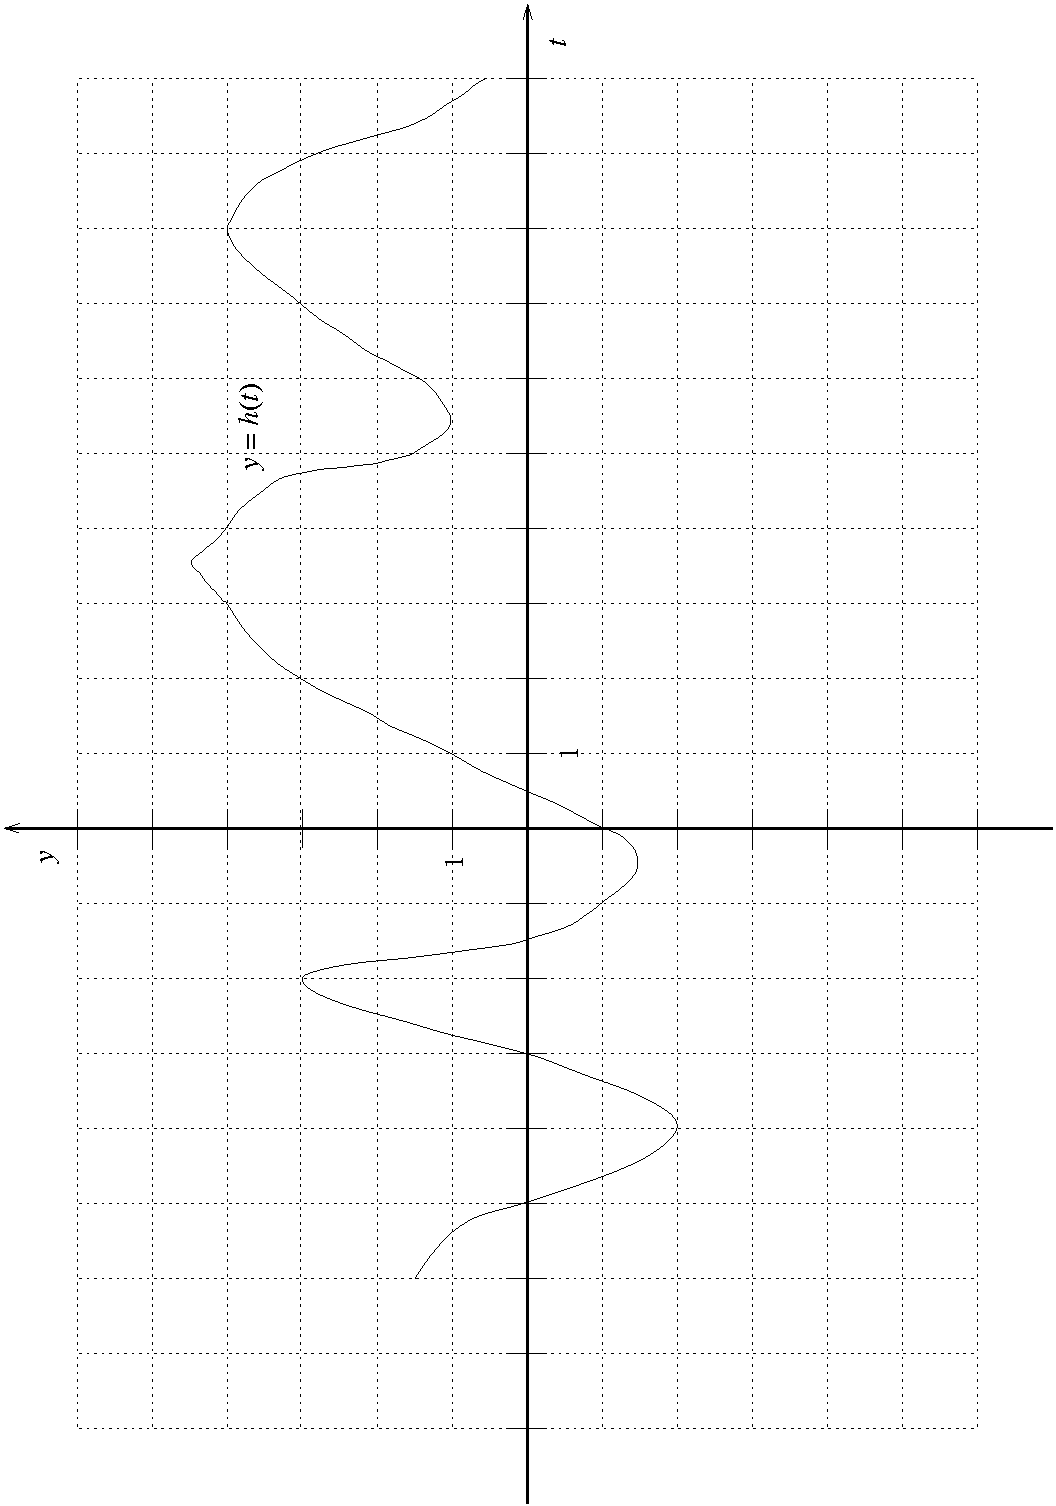
\includegraphics[angle=270,scale=0.85]{graphicDetails.pdf}
}

\end{document}
